\section{Implementation:}\label{sec:implementation}

%%%%%%%%%%%%%%%%%%%%%%%%%%%%%%%%%%%%%%%%%%%%%%
% ESP-Now Mesh (SLAVE) - Ben
%%%%%%%%%%%%%%%%%%%%%%%%%%%%%%%%%%%%%%%%%%%%%%
% ESP-NOW mesh diagram %
\subsection{ESP-Now Mesh}\label{sec:espnowmesh}
\begin{figure}[H]
  \begin{center}
    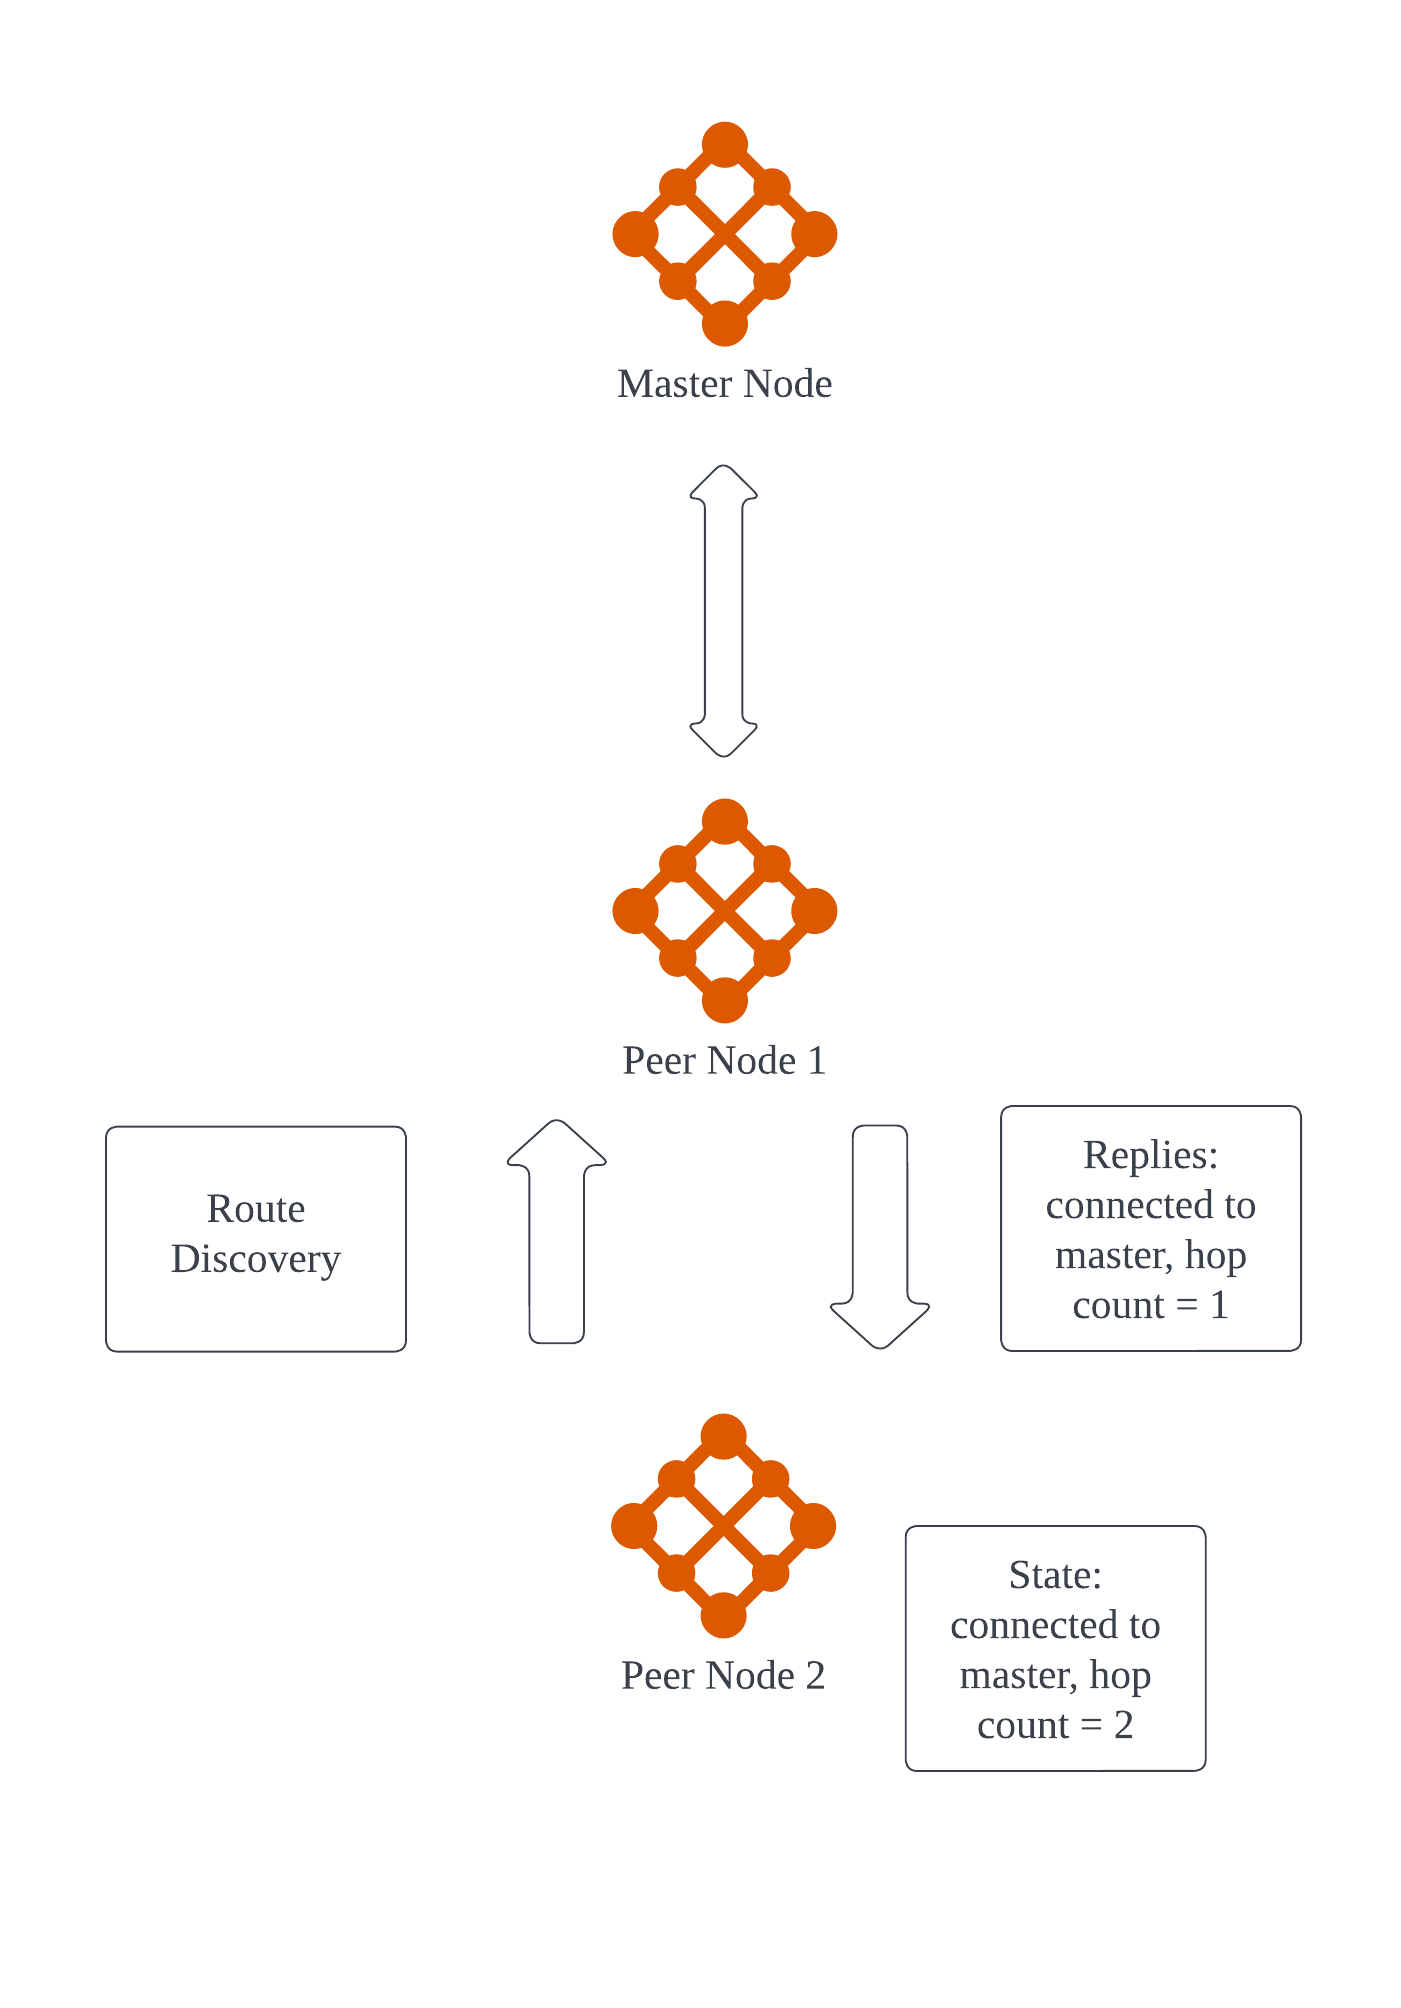
\includegraphics[width=0.14\textwidth]{./Figures/ESP-NOW/espnow_join_mesh.png}
    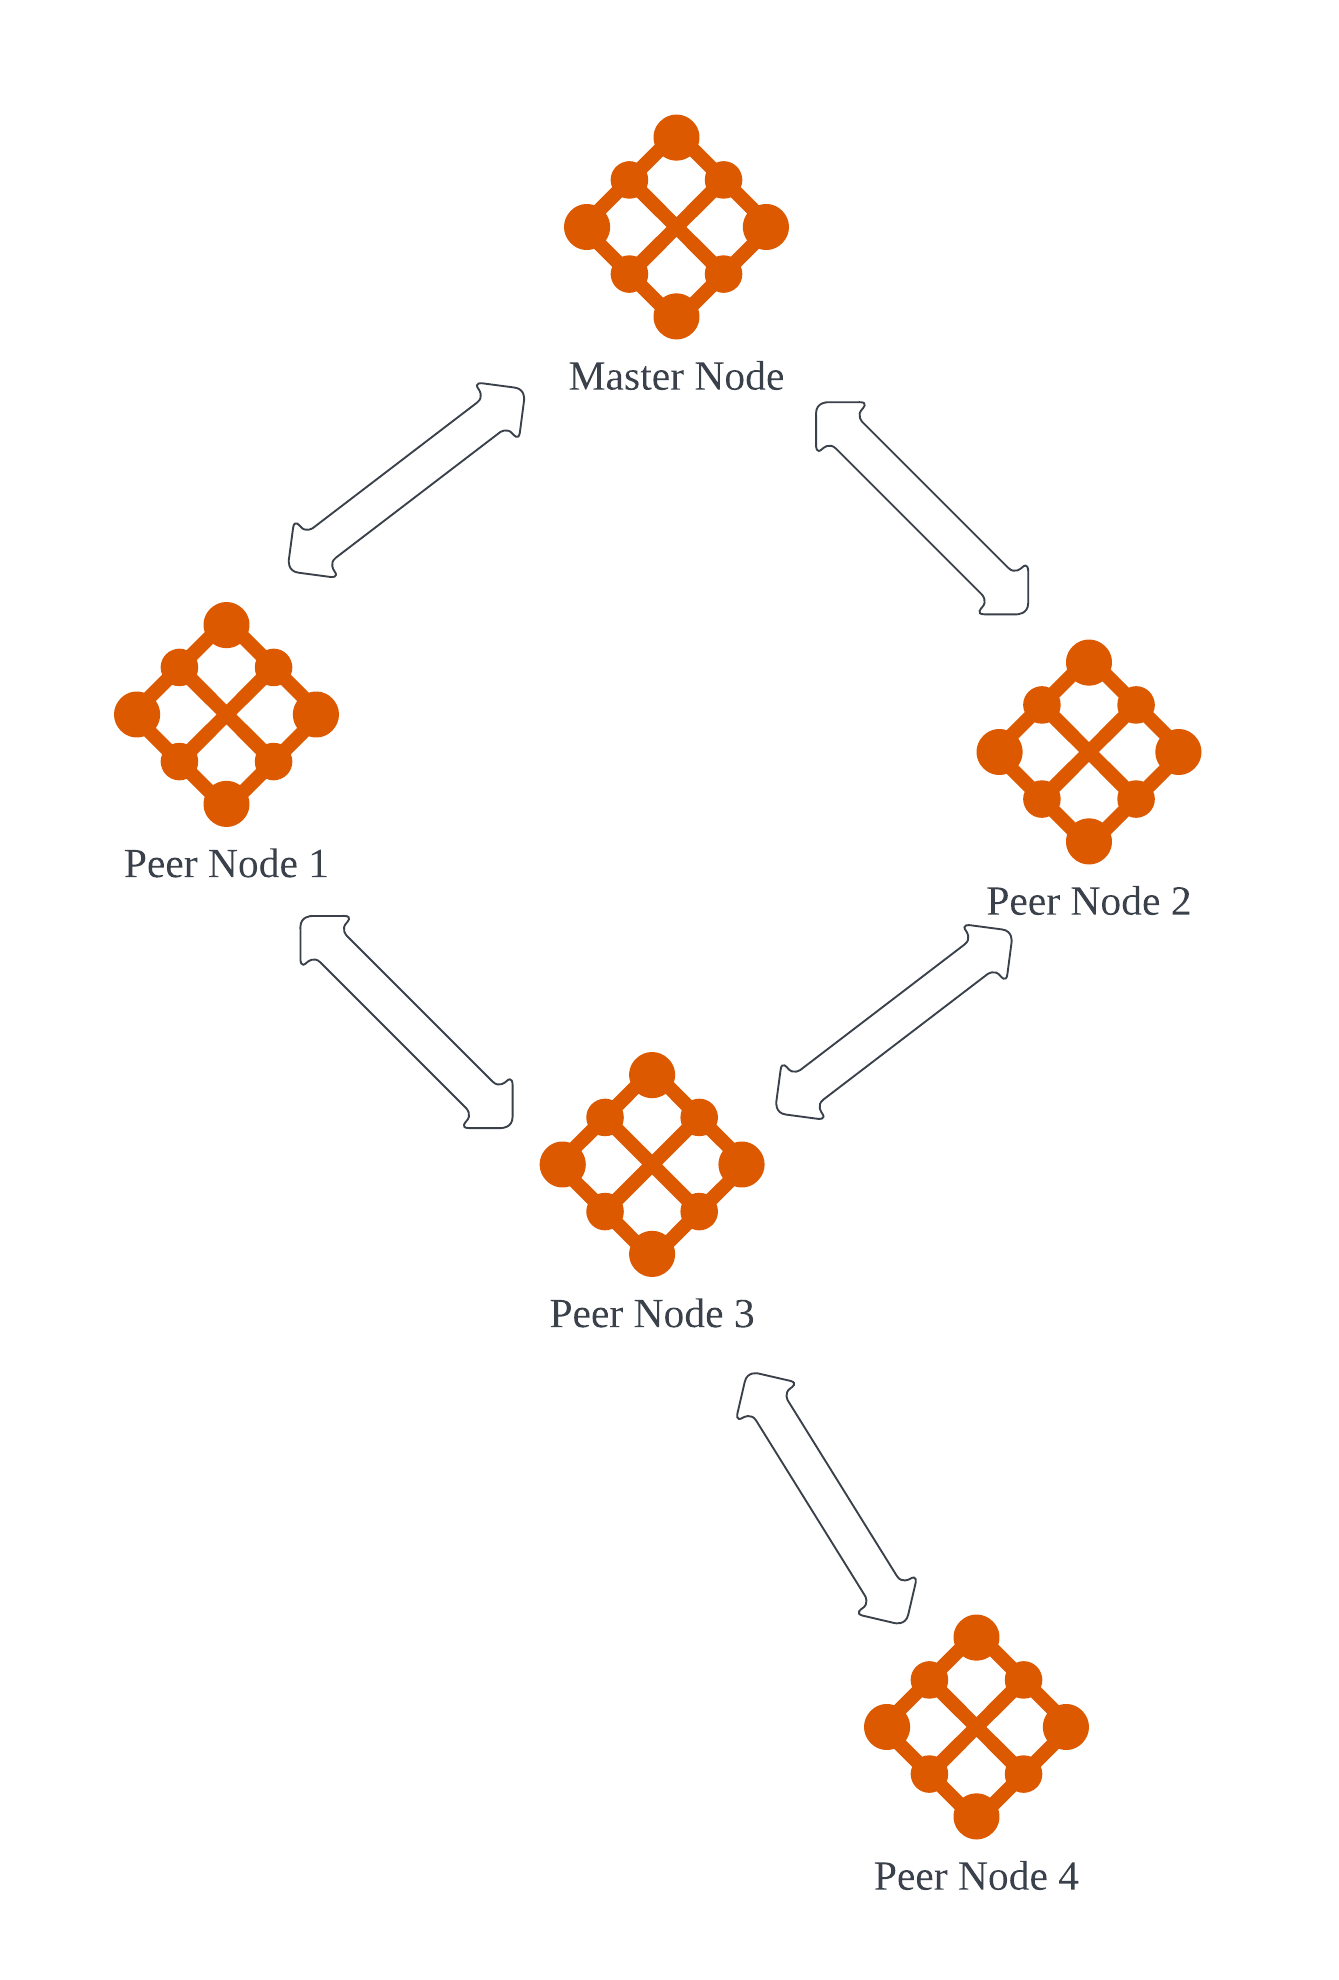
\includegraphics[width=0.14\textwidth]{./Figures/ESP-NOW/espnow_data_transfer.png}
  \end{center}
  \caption{ESP-NOW Nodes joining network \& data transfer}\label{espnow_data_transfer}
\end{figure}

The ESP-Now Mesh implementation adopts a tailored version of the Dynamic Source Routing (DSR) mesh algorithm, designed specifically for environmental monitoring applications. This algorithm optimizes route building and peer node deployment for real-world scenarios. The mesh algorithm assumes the best case approach when it comes to building routes along with the careful considerations of deployment of peer nodes in real life. Within this network, it assumes that there is an initial precense of a Master node and each peer node keeps a record of nearby nodes capable of reaching the master node, leveraging the peer list feature of the ESP-NOW library. When a node needs to send data collected from the SCD41 sensor but lacks the route information to the master, it initiates the route discovery process by sending out a handshake packet to its immediate neighbors. Upon receiving this packet, if a neighbor knows the path to the master, it responds by indicating its route knowledge and hop count. The originating node then updates its routing information, registers the responding peer’s MAC address into its list, and proceeds to transmit the data either directly to the master node or through peers that have a known route to the master. 

The deployment strategy for this mesh network emphasizes optimal node positioning to prevent data redundancy and congestion. Nodes needs to be strategically placed to avoid collecting redundant data and to minimize the inclusion of redundant peers in their peer lists. This approach aims to ensure that each area of deployment ideally contains only 1-2 nodes. Nodes are configured to include only peers that are closer to the master in their peer lists, as the route building in this algorithm progresses upwards towards the master node. This strategy helps reduce the number of redundant and repeated packets transmitted in the mesh network, thereby optimizing network performance and efficiency.

%%%%%%%%%%%%%%%%%%%%%%%%%%%%%%%%%%%%%%%%%%%%%%
% LORA Mesh (SLAVE) - Richie
%%%%%%%%%%%%%%%%%%%%%%%%%%%%%%%%%%%%%%%%%%%%%%
%insert diagram here%
\subsection{LoRa Mesh}\label{sec:loramesh}
\begin{figure}[H]
  \begin{center}
    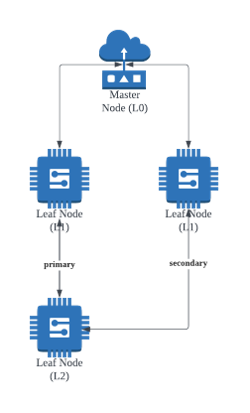
\includegraphics[width=0.14\textwidth]{Figures/LoRa/lora_structure_1.png}
    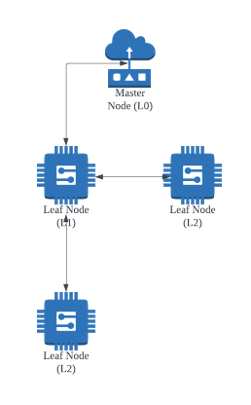
\includegraphics[width=0.14\textwidth]{Figures/LoRa/lora_structure_2.png}
  \end{center}
  \caption{LoRa Nodes joining network \& data transfer}
\end{figure}

%hierarchy architecture
The LoRa Mesh is implemented with a modified DSR with hierarchy architecture design. Nodes are ranked by their hop count towards the master node, whereby nodes further away from the master node holds a higher rank value. This architecture design allows the nodes to store only the addresses of the nodes of lower rank value, instead of the traditional way whereby nodes store the routes to destination. The flooding effect during route discovery can be mitigated as the discovery messages will only be propagated once per discovery. 
%packet type - discovery
In order to build a mesh network, the route table, discovery and reply messages are needed. The discovery message is the simplest message format, which contains only the message type. Nodes will regularly check its route table, if it is empty, the discovery message will be sent. Nodes that receive the discovery message will check whether its own route table is empty, if it is not, it will reply the discovery message with its own MAC address and rank. Other nodes that receive the dicovery reply message, regardless if it has started a discovery, will update its route table if applicable. As such, the route table will be regularly updated with the nearest nodes with the lowest rank.
%packet type - data
The primary objective of the nodes are for environmental data collection and transmission. Therefore, when a data packet is generated by the sensor or is received from the other nodes, the leaf nodes will forward the data packet to a lower rank node in the route table. The data packet, other than the sensor data, contains the MAC address of the original sender, the MAC address of the next receiver and a random generated number for verification. When forwarding, nodes will change the MAC address that indicates the next receiver to the first address of its route table. Upon receiving a data packet successfully, the node will reply back to the previous sender immediately. The reply message, typically contains the message type and the random number from the corresponding data packet. When the node that sends out the data packet receives the reply, it will check the random number against the record to determine if the reply correct. This was designed for nodes to be able to listen out for multiple reply packets. However, due to the constraint of the LoRa module, the nodes will only listen for one reply message at a time. As LoRa does broadcast communicaiton only, nodes will receive data packets that are not intended for them, and are unable to tell if the data packets sent are successfully received by the receiver node. Therefore, the data reply mechanism is implemented to ensure important data packets are received at least once.
%queues
The LoRa module only can receive or transmit one data packet at a time. As a result, messages cannot be reliably transmitted. To resolve this issue, data queues are implemented for data receiving, data to send and data sending. Because the main loop of the system is running in single thread, data receiving will be prioritised. As such, multiple data packets can be received and directly stored in the receiving queue before any filtering or processing. In the ideal situation, it will process the queued data packets from the queue. When data packet that requires a reply is sent, it will the packet be removed from the queue; if the reply is not received after a certain duration, the data packet in the sending queue will be moved back to the data to send queue again. Moreover, packets that does not require a reply, such as the reply packets, will be prioritised by placing them at the start of the queue to prevent deadlocks.
%timeout and retry
Network interrupt handling is one of the greatest strength of the DSR protocol. Whenever a data reply is not received after a fixed duration, it will retry up to three times, before switching to the next address in the route table. As the data packets are all stored in a queue, there will be lesser chance of having missed a data packet, although it poses a potential risk of buffer overflow. If the error occurs too many times, it will attempt to switch to use ESP-NOW mesh to maintain the connectivity.
%conclusion - robust, swiftness, efficient
This LoRa implementation approach showcases the robustness, swiftness, and efficiency in environmental data transmission. Its design significantly reduces the complexity of route tables and mitigates the flooding effect, enhancing network reliability. With swift data packet handling through prioritized queues and a retry mechanism, it ensures data integrity and timely responses, even with the single-thread limitations of the LoRa module. 

%%%%%%%%%%%%%%%%%%%%%%%%%%%%%%%%%%%%%%%%%%%%%%
% Master Node Stack
%%%%%%%%%%%%%%%%%%%%%%%%%%%%%%%%%%%%%%%%%%%%%%
\subsection{Master Node Infrastructure}\label{sec:master}

The Master Node Infrastructure encompasses a suite of pivotal components meticulously designed to harmoniously facilitate the monitoring and management of IoT devices. Charged with duties spanning data aggregation, processing, and user interface provisioning, the Master Node assumes a central role in orchestrating system functionalities. Core elements of this infrastructure comprise the Liligo Gateway, a Raspberry Pi MQTT Client and Broker, and the ELK Stack. Furthermore, our implementation integrates a router to establish an artificial cloud-based server for the ELK Stack.

\subsubsection{Protocol Master}\label{sec:protocol}

Serving as the protocol master within the Master Node setup, the Liligo Module shoulders the vital responsibilities of traffic monitoring, serialization, and MQTT-based transmission to the ELK stack. In collaboration with a Raspberry Pi configured as both MQTT Client and Broker, the Liligo Module establishes a USB connection for seamless data transfer to the Raspberry Pi. Subsequently, the Raspberry Pi orchestrates the dissemination of serialized data to the ELK stack via MQTT.

Configured to monitor Lora and ESP-Now Protocol packets, the Liligo Module acts as the primary data acquisition unit. Upon reception, data undergoes serialization and is then forwarded to the MQTT Broker by the Raspberry Pi 4b, facilitating streamlined integration with the ELK stack for subsequent processing.

\subsubsection{ELK Stack}\label{sec:elk}
% Backbone Cloud-based server Stack
\begin{figure}[H]
  \begin{center}
    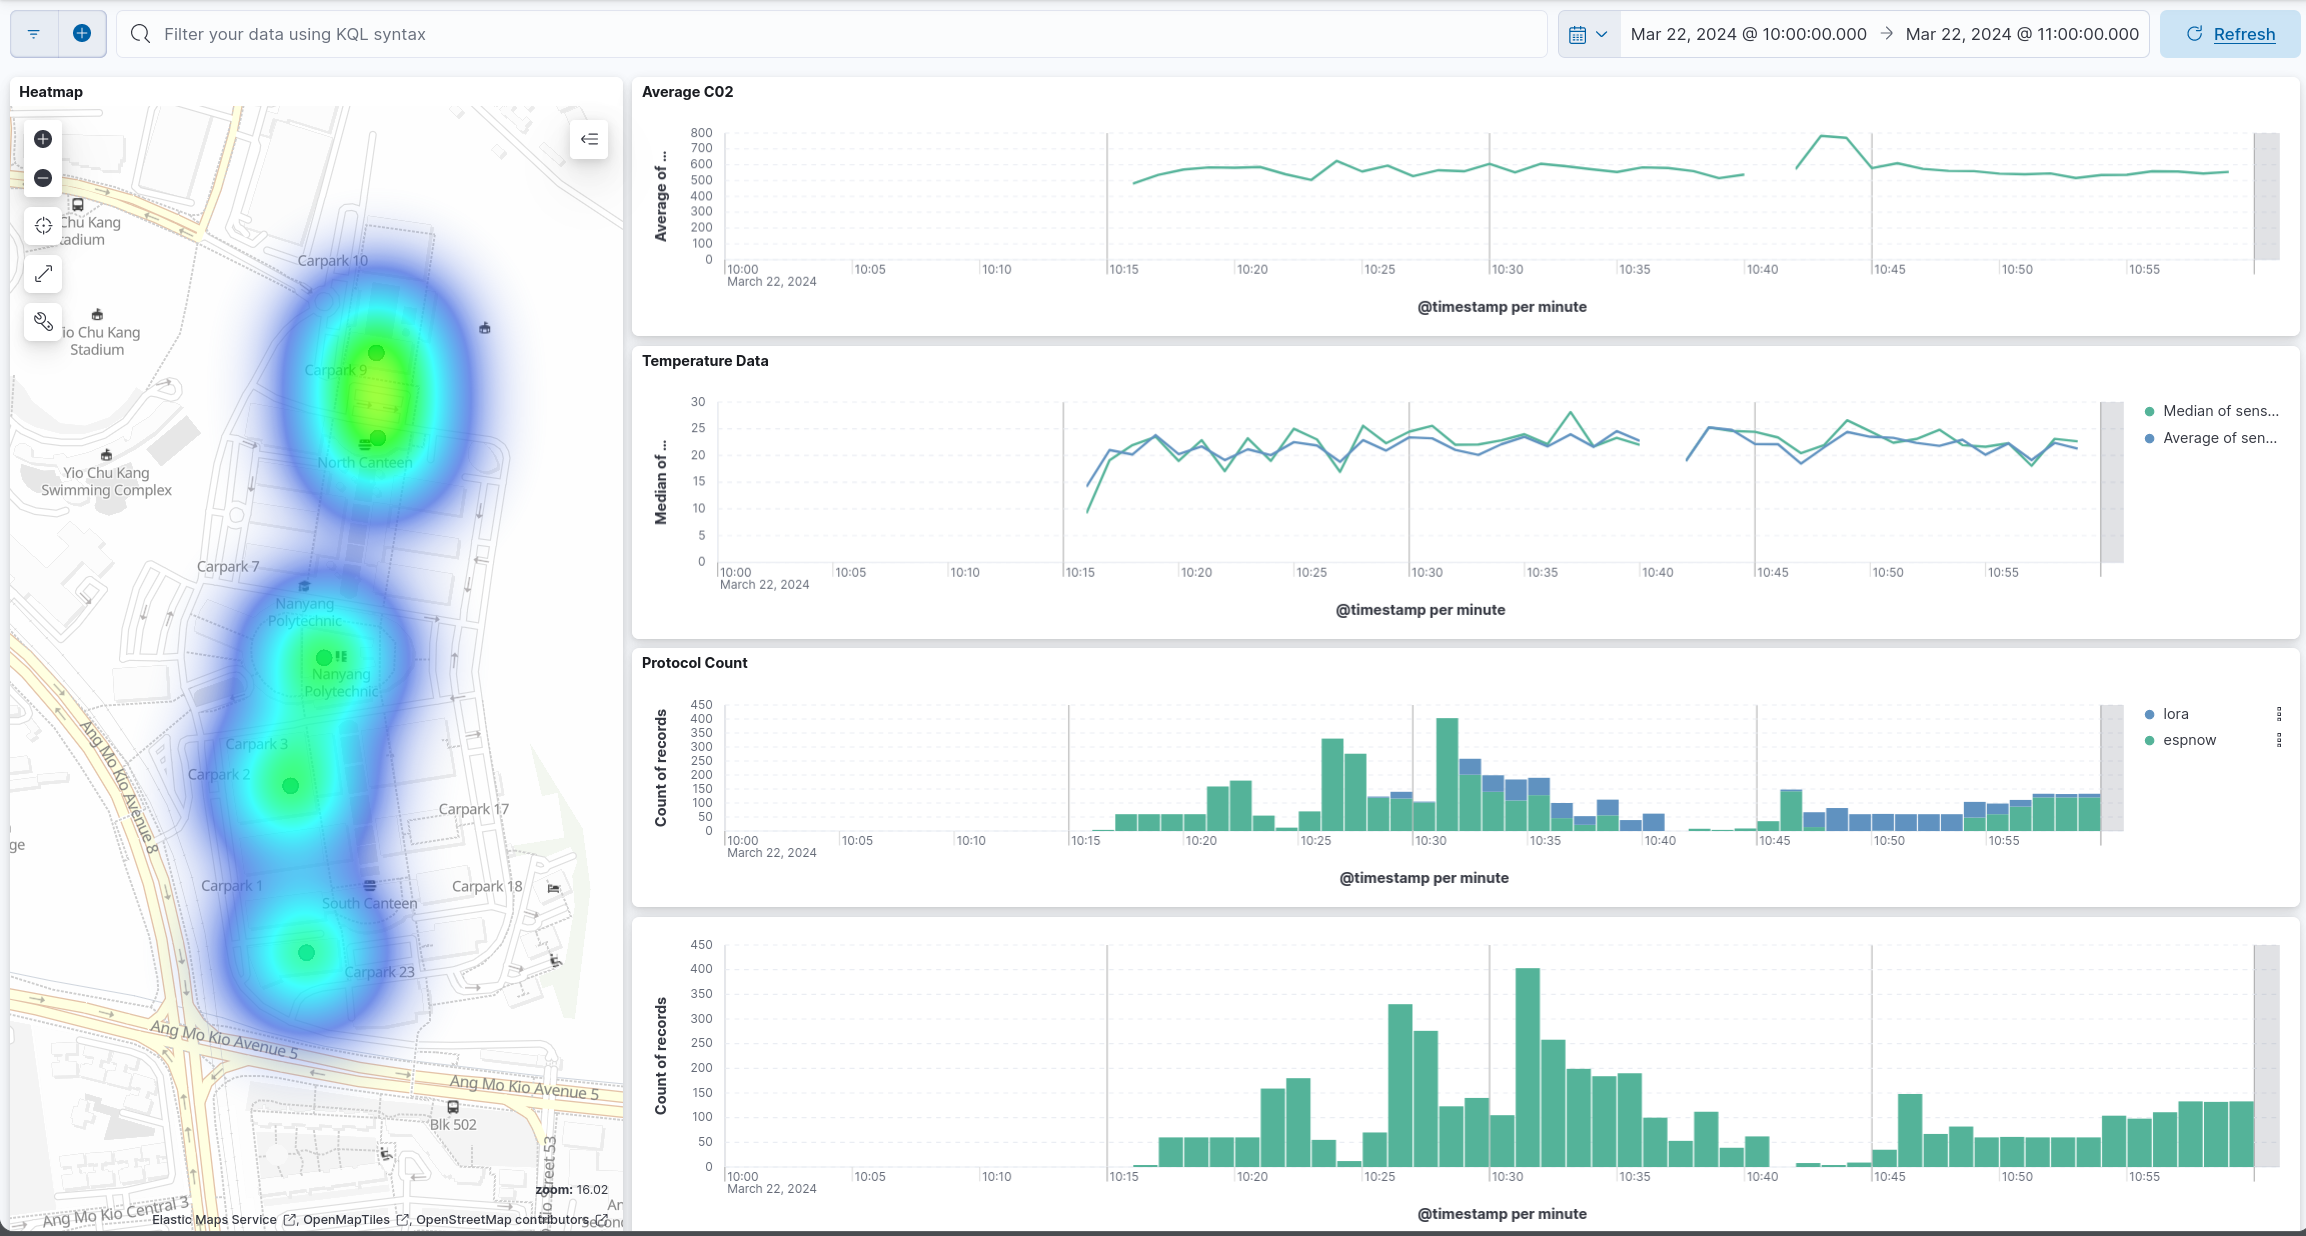
\includegraphics[width=0.35\textwidth]{./Figures/elk/elk_dashboard.png}
  \end{center}
  \caption{ELK Dashboard}\label{fig:elk_dashboard}
\end{figure}

The deployment of the ELK Stack is streamlined through the utilization of Docker and Docker Compose, enabling efficient deployment with minimal configuration overhead. Comprising Elasticsearch, Logstash, and Kibana, the ELK Stack offers a robust framework for data storage, processing, and visualization. Elasticsearch, a distributed, RESTful search and analytics engine, serves as the cornerstone for storing extensive datasets. Logstash functions as a versatile data processing pipeline, ingesting data from diverse sources, transforming it, and then forwarding it to a designated "stash" such as Elasticsearch. Kibana, a powerful data visualization dashboard, empowers users to interact with and explore data stored in Elasticsearch.

Raw data emanating from the Liligo Module is routed to the Raspberry Pi before being relayed to the ELK stack for processing. Following processing, data is stored within Elasticsearch. Kibana is subsequently employed to create visualization dashboards, offering insights into various metrics such as packet transmission, environmental parameters, device connectivity, and protocol distribution.

These visualizations furnish valuable insights facilitating the monitoring of the Wireless Sensor Network (WSN), enabling performance evaluation of protocol switching. This analysis, outlined in Section \ref{sec:analysis}, encompasses metrics including packet transmission, environmental data, device connectivity, protocol distribution, and power consumption analysis.

\subsubsection{Switching}\label{sec:switching}

A pivotal feature ingrained within all slave nodes is the capability to seamlessly transition between the LORA and ESP-Now protocols in response to evolving network dynamics. This feature assumes paramount significance in the comprehensive evaluation of each protocol's efficacy across diverse network conditions. The switching mechanism, autonomously activated by individual slave nodes, predicates its decision on the observed packet failure rate. Upon discerning a notable uptick in packet failures, the slave node instigates a judicious transition to the alternative protocol. Such a mechanism stands as a linchpin in preserving network robustness and fostering optimal performance amidst fluctuating network exigencies.

An inherent advantage of this mechanism lies in its facilitation of comparative performance assessments between the two protocols amidst varying network topologies and conditions. By juxtaposing their respective performance metrics, stakeholders can glean invaluable insights into the aptness of each protocol for specific application scenarios contingent upon the prevailing network milieu. Moreover, the dynamic switching functionality serves as a potent tool for pinpointing the protocol best suited to a given network configuration, thereby engendering heightened network efficiency and reliability.

A visual representation of the switch is depicted in Figure \ref{fig:protocol_distribution}




